\section{RenderDoc 截帧记录}
这次捕获使用 32×32 的回归用例，底色贴图 alpha、独立透明度图红通道和 0.75 材质因子相乘，裁剪阈值为 0.5。它先画深度，再清屏独立画主画面，捕获范围只有这个用例。

捕获由 RenderDoc 1.33 的应用接口完成，使用 1.47 回放。设备为 RTX 5070 Ti Laptop GPU，OpenGL 4.6，NVIDIA 驱动 616.56。下图是实际 RenderDoc 界面，不是测试程序另行生成的结果图。

\begin{figure}[H]
\centering
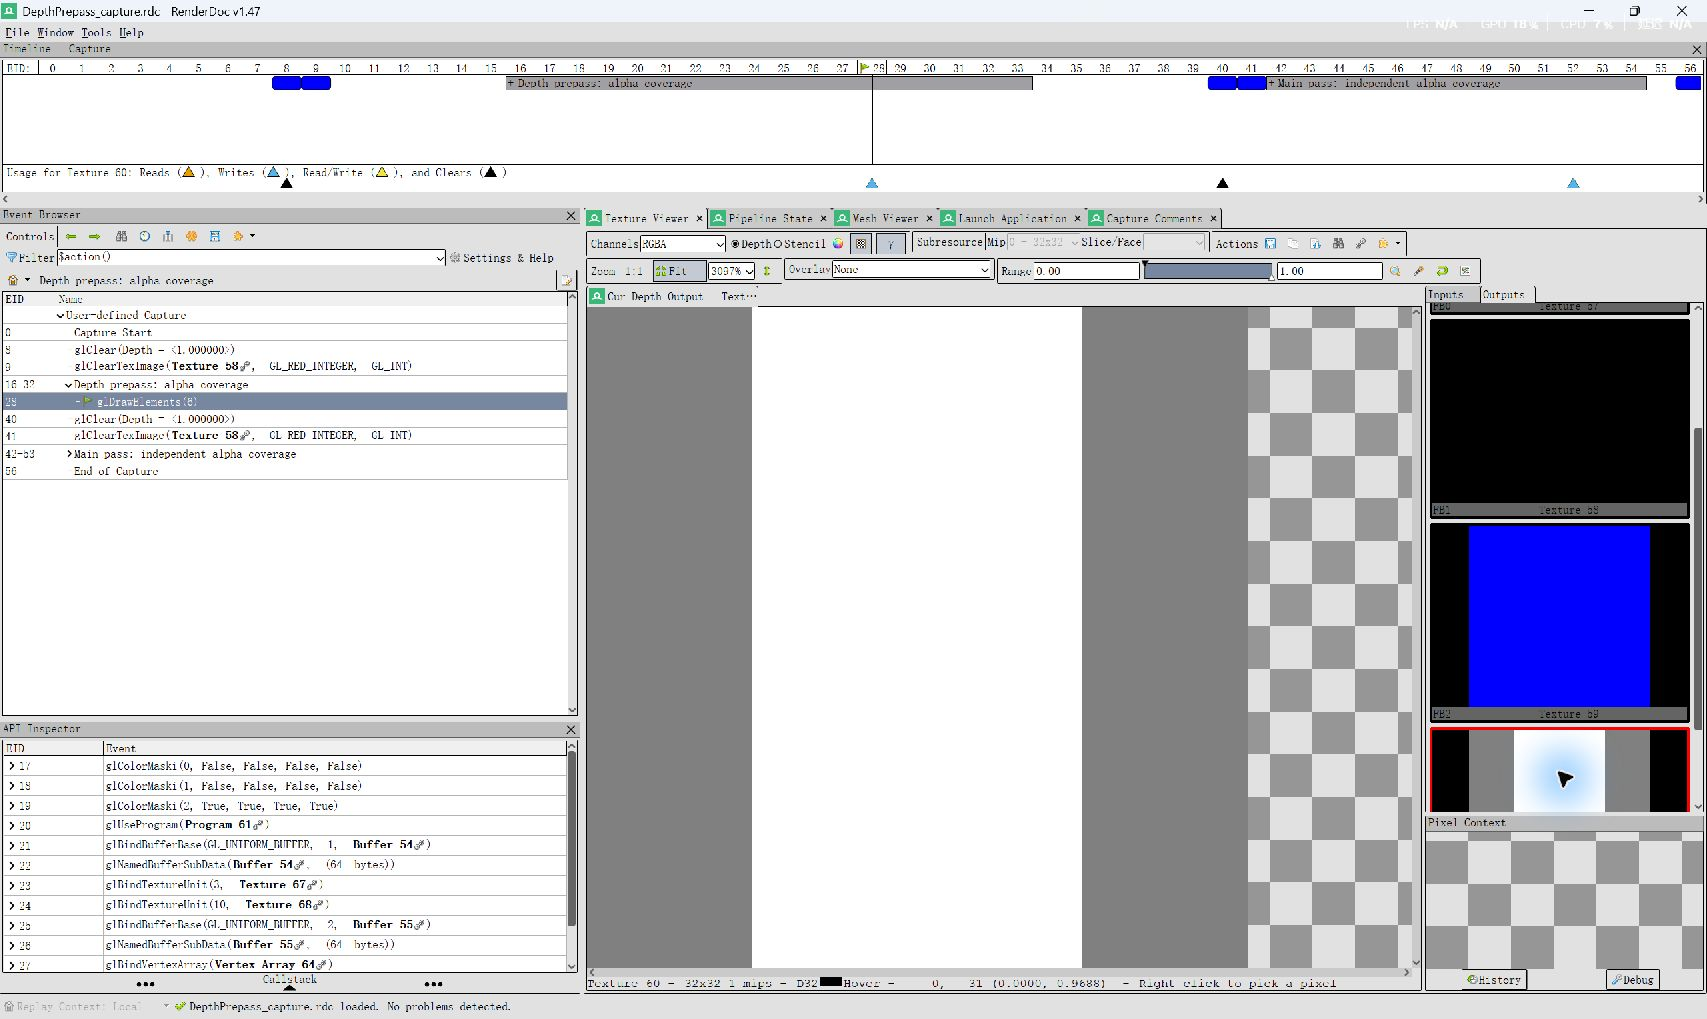
\includegraphics[width=\linewidth]{../../../output/captures/renderdoc-eid28-depth.jpg}
\caption{选中事件编号 EID 28 的深度预传递，Texture 60 为 D32 深度附件；两侧灰色为写入区域，中间白色保留清屏深度}
\end{figure}

回放定位到两次六索引绘制：EID 28 为深度预传递，EID 52 为主绘制。两者使用同一深度附件，中间有独立清屏。下表通过 RenderDoc 的 PickPixel 读取，坐标原点为左上，均位于 $y=16$。

\begin{tabularx}{\textwidth}{L{4.4cm}YYY}
\toprule
事件与附件 & $x=4$ & $x=12$ & $x=28$ \\
\midrule
EID 28，深度 & 0.5 & 1.0 & 0.5 \\
EID 52，深度 & 0.5 & 1.0 & 0.5 \\
EID 28，实体 ID & -1 & -1 & -1 \\
EID 52，实体 ID & 42 & -1 & 42 \\
\bottomrule
\end{tabularx}

全部 1024 个像素也已核对，两次绘制后的深度数据逐字节相同。512 个像素为 0.5，其余为 1.0。预传递不写实体 ID，因此全部保留 -1。主绘制在保留区域写入 42。六组自动测试另行覆盖更多开关组合。

捕获中还有 14 条信息消息和 1 条 NVIDIA 驱动性能提示：EID 28 的顶点着色器依据 GL 状态重新编译。回放开启 API 验证后只有 3 条信息消息，未报致命错误。尚未测量该重编译的持续时间和重复频率，不能写成零告警或已找到性能瓶颈。

\note{原始捕获：\path{output/captures/DepthPrepass_capture.rdc}，59936 字节。SHA-256 前缀为 \code{3dcc81ca9eb3ba44}，完整值与回放记录见同目录 manifest.json、replay-results.json。尚未测量 GPU 耗时。}
